% verso e anverso:
% \documentclass[12pt,openright,twoside,a4paper,english]{abntex2}
% apenas verso:	
\documentclass[12pt,oneside,a4paper,english]{abntex2} 

\usepackage[alf]{abntex2cite}	% Citações padrão ABNT
\usepackage{listings}
\usepackage{float}
\usepackage{cmap}				% Mapear caracteres especiais no PDF
\usepackage{lmodern}			% Usa a fonte Latin Modern			
\usepackage[T1]{fontenc}		% Selecao de codigos de fonte.
\usepackage[utf8]{inputenc}		% Codificacao do documento (conversão automática dos acentos)
\usepackage{lastpage}			% Usado pela Ficha catalográfica
\usepackage{indentfirst}		% Indenta o primeiro parágrafo de cada seção.
\usepackage{color}				% Controle das cores
\usepackage{graphicx}			% Inclusão de gráficos
\usepackage{pdfpages}
\usepackage{tikz}
\usetikzlibrary{automata,positioning}
\usepackage{mathtools}

\definecolor{blue}{RGB}{41,5,195} % alterando o aspecto da cor azul

\makeatletter
\hypersetup{
    %pagebackref=true,
    pdftitle={\@title}, 
    pdfauthor={\@author},
    pdfsubject={\@title},
    pdfcreator={\imprimirpreambulo},
    pdfkeywords={Linguagens}{Compiladores}{Relatório Final}, 
    colorlinks=true,       		% false: boxed links; true: colored links
    linkcolor=blue,          	% color of internal links
    citecolor=blue,        		% color of links to bibliography
    filecolor=magenta,      		% color of file links
    urlcolor=blue,
    bookmarksdepth=4
}
\makeatother

\autor{Gustavo P. Gouveia (6482819), Victor Lassance (6431325)}
\title{Relatório de Compiladores\\Relatório Final\\Linguagem de programação \underline{CZAR}}
\orientador[Professor:]{Ricardo Luis de Azevedo da Rocha}
\preambulo{Texto apresentado à Escola Politécnica da Universidade de São Paulo como requisito para a aprovação na disciplina Linguagens e Compiladores no quinto módulo acadêmico do curso de graduação em Engenharia de Computação, junto ao Departamento de Engenharia de Computação e Sistemas Digitais (PCS).}
\instituicao{%
	Universidade de São Paulo
	\par
	Escola Politécnica
	\par
	Engenharia de Computação - Curso Cooperativo}
\local{São Paulo}
\data{2013}
\tipotrabalho{PCS2056 - Linguagens e Compiladores}

\setlength{\parindent}{1.3cm} % O tamanho do parágrafo
\setlength{\parskip}{0.2cm}  % Controle do espaçamento entre um parágrafo e outro
\lstset{basicstyle=\footnotesize\ttfamily}
\makeindex

\begin{document}

\frenchspacing % Retira espaço extra obsoleto entre as frases.

\imprimirfolhaderosto

\tableofcontents

\textual

\chapter{Introdução}
\label{chap:introducao}
	% !TEX encoding = UTF-8 Unicode

Este projeto tem como objetivo a construção de um compilador de um só passo, dirigido por sintaxe, com analisador e reconhecedor sintático baseado em autômato de pilha estruturado.

Em um primeiro momento, foi definida uma linguagem de programação e identificados os tipos de átomos. Para cada átomo foi escrito uma gramática linear representativa da sua lei de formação e um reconhecedor para o átomo. Desse modo, as gramáticas assim escritas foram unidas e convertidas em um autômato finito, o qual foi transformado em um transdutor e implementado como sub-rotina, dando origem ao analisador léxico propriamente dito. Também foi criada uma função principal para chamar o analisador léxico e possibilitar o seu teste.

Durante a segunda etapa, a sintaxe da linguagem, denonimada por nós de CZAR, foi definida formalmente a partir de uma definição informal e de exemplos de programas que criamos, misturando palavras-chave e conceitos de diferentes linguagens de programação. As três principais definições foram escritas na notação BNF\footnote{Ver http://en.wikipedia.org/wiki/Backus\_Naur\_Form}, Wirth\footnote{Ver http://en.wikipedia.org/wiki/Wirth\_syntax\_notation} e com diagramas de sintaxe.

Na terceira etapa, implementamos o módulo referente à parte sintática para a nossa linguagem. O analisador sintático construído obtém uma cadeia de \emph{tokens} proveniente do analisador léxico, e verifica se a mesma pode ser gerada pela gramática da linguagem e, com isso, constrói a árvore sintática \cite{alfred1986compilers}.

Para a quarta entrega, focamos no ambiente de execução. O compilador por nós criado tem como linguagem de saída um programa que é executado na máquina virtual conhecida como Máquina de von Neumann (MVN).

Já durante as duas últimas entregas, complementamos a especificação do código gerado pelo compilador e das rotinas do ambiente de execução da nossa linguagem de alto nível, a CZAR. Além disso, buscamos integrar as rotinas semânticas no reconhecedor sintático de forma a permitir a geração de código e finalizar o compilador.

Como material de consulta, além de sites sobre o assunto e das aulas ministradas, foi utilizado o livro indicado pelo professor no começo das aulas \cite{intro-compiladores}, para pesquisa de conceitos e possíveis implementações.

O documento apresenta a seguir o processo completo de desenvolvimento de um compilador, desde a definição formal da linguagem, passando pelo analisador léxico, reconhecedor sintático, pela definição do ambiente de execução e das rotinas semânticas, terminando com um exemplo de programa traduzido.


\chapter{Definição da linguagem}
\label{chap:definicao}
	% !TEX encoding = UTF-8 Unicode

\section{Descrição Informal da Linguagem}
\label{sec:desc-informal}

O programa é composto por quatro partes, explicadas abaixo de forma 
simplificada, pois a linguagem será definida de forma completa nas seções~\ref{sec:bnf} e~\ref{sec:wirth} nas notações \verb!BNF! e
\verb!Wirth!, respectivamente:

\begin{itemize}
    \item Definição do programa:
            
            Um programa em \verb!czar! possui em ordem obrigatória, a
            importação de bibliotecas, declaração de variáveis globais,
            definição de funções e procedimentos. O programa deve terminar
            obrigatoriamente pela declaração da função principal \verb!main!.

        \begin{itemize}
            \item \verb$PROGRAM = IMPORTS DECLS_GLOBAIS DEF_PROCS_FUNCS DEF_MAIN.$
        \end{itemize}
    \item Inclusão de bibliotecas:
        \begin{itemize}
            \item \verb$IMPORTS = { `<' IDENT `>' }.$
        \end{itemize}
    \item Declaração de tipos, variáveis e constantes de escopo global:
        \begin{itemize}
            \item \verb$DECLS_GLOBAIS = { DEF_TIPO | DECL }.$
            \item \verb$DEF_TIPO = `struct' IDENT `{' { DECL } `}'.$
            \item \verb$DECL = [ `const' ] TIPO IDENT [ `=' EXPR ]$\\
                    \verb${ `,' IDENT [ `=' EXPR ] } `;'.$
        \end{itemize}
    \item Definição dos procedimentos e funções do programa, 
        As funções não devem incluir o procedimento principal (chamado
        \verb!main!). Estas também possuem retorno final único e obrigatório. 
        \begin{itemize}
            \item \verb$DEF_PROCS_FUNCS = { PROC | FUNC }.$
            \item \verb$FUNC = TIPO IDENT LIST_PARAMS$\\
                    \verb$`{' { INSTR_SEM_RET } "return" EXPR [ ";" ] `}'.$
            \item \verb$PROC = `void' IDENT LIST_PARAMS `{' { INSTR_SEM_RET } `}'.$
            \item \verb$LIST_PARAMS = `(' [ [ `ref' ] TIPO IDENT ]$\\
                    \verb${ `,' [ `ref' ] TIPO IDENT } `)'.$
        \end{itemize}
    \item Definição do procedimento principal (chamado \verb!main!):
            
            Não existe
            passagem explícita de parâmetros para a função \verb!main!, ou seja,
            a passagem de valores para a mesma deve ocorrer por meio de
            arquivos ou pela utilização de uma função incluida por alguma
            biblioteca \emph{built-in} a ser feita, permitindo o acesso dos
            parâmetros em todas as partes do código. 
        \begin{itemize}
            \item \verb$DEF_MAIN = `main' `(' `)' `{' [ BLOCO ] `}'.$
        \end{itemize}
\end{itemize}

\section{Descrição da Linguagem em BNF}
\label{sec:bnf}

Apesar de termos visto em aula que a sintaxe BNF não costuma ter os não-terminais explicitados entre aspas, prefirimos colocar aspas simples para facilitar a leitura, que também é uma forma válida de sintaxe BNF\footnote{Ver http://www.cs.man.ac.uk/~pjj/bnf/bnf.html}.

\begin{lstlisting}[frame=single,numbers=left,breaklines=true,mathescape=true>,basicstyle=\ttfamily\scriptsize]
<PROGRAM>            ::= <IMPORTS> <DECLS_GLOBAIS> <DEF_PROCS_FUNCS> <DEF_MAIN>

<IMPORTS>            ::= $\epsilon$
                       | '<' <IDENT> '>' <IMPORTS>

<DECLS_GLOBAIS>      ::= $\epsilon$
                       | <DEF_TIPO> <DECLS_GLOBAIS>
                       | <DECL_CONST> <DECLS_GLOBAIS>
                       | <DECL_VAR> <DECLS_GLOBAIS>  

<DEF_TIPO>           ::= 'struct' <IDENT> '{' <DEF_INSTR_TIPO> '}'

<DEF_INSTR_TIPO>     ::= $\epsilon$
                       | <DECL_CONST>
                       | <DECL_VAR>

<DECL_CONST>         ::= 'const' <DECL_VAR>

<DECL_VAR>           ::= <TIPO> <IDENT> <DECL_VAR_CONT> ';'
                       | <TIPO> <IDENT> '=' <EXPR> <DECL_VAR_CONT> ';'

<DECL_VAR_CONT>      ::= $\epsilon$
                       | ',' <IDENT> <DECL_VAR_CONT>
                       | ',' <IDENT> '=' <EXPR> <DECL_VAR_CONT>

<DEF_PROCS_FUNCS>    ::= $\epsilon$
                       | <PROC> <DEF_PROCS_FUNCS>
                       | <FUNC> <DEF_PROCS_FUNCS>

<FUNC>               ::= <TIPO> <IDENT> <LIST_PARAMS> '{' <INSTRUCOES> 'return' <EXPR> '}'
                       | <TIPO> <IDENT> <LIST_PARAMS> '{' <INSTRUCOES> 'return' <EXPR> ';' '}'

<PROC>               ::= 'void' <IDENT> <LIST_PARAMS> '{' <INSTRUCOES> '}'

<INSTRUCOES>         ::= $\epsilon$
                       | <INSTR_SEM_RET> <INSTRUCOES>

<LIST_PARAMS>        ::= '(' ')'
                       | '(' <TIPO> <IDENT> <LIST_PARAMS_CONT> ')'
                       | '(' 'ref' <TIPO> <IDENT> <LIST_PARAMS_CONT> ')'

<LIST_PARAMS_CONT>   ::= $\epsilon$
                       | ',' <TIPO> <IDENT> <LIST_PARAMS_CONT>
                       | ',' 'ref' <TIPO> <IDENT> <LIST_PARAMS_CONT>

<DEF_MAIN>           ::= 'main' '(' ')' '{' <INSTRUCOES> '}'

<INSTR_SEM_RET>      ::= <DECL_VAR>
                       | <ATRIB>
                       | <PROC_CALL>
                       | <FLOW_CONTROL>

<ATRIB>              ::= <ATRIB_SEM_PV> ';'

<ATRIB_SEM_PV>       ::= <VARIDENT> <OPER_ATRIB> <EXPR> <ATRIB_SEM_PV_CONT>

<ATRIB_SEM_PV_CONT>  ::= $\epsilon$
                       | ',' <VARIDENT> <OPER_ATRIB> <EXPR> <ATRIB_SEM_PV_CONT>

<PROC_CALL>          ::= <IDENT> '(' ')' ';'
                       | <IDENT> '(' <EXPR> <PROC_CALL_CONT> ')' ';'

<PROC_CALL_CONT>     ::= $\epsilon$
                       | ',' <EXPR> <PROC_CALL_CONT>

<FLOW_CONTROL>       ::= <FOR_CONTROL>
                       | <WHILE_CONTROL>
                       | <IF_CONTROL>

<FOR_CONTROL>        ::= 'for' '(' <DECL_VAR> <COND> ';' <ATRIB_SEM_PV> ')' '{' <INSTRUCOES> '}'

<WHILE_CONTROL>      ::= 'while' '(' <COND> ')' '{' <INSTRUCOES> '}'

<IF_CONTROL>         ::= 'if' '(' <COND> ')' '{' <INSTRUCOES> '}'
                       | 'if' '(' <COND> ')' '{' <INSTRUCOES> '}' 'else' '{' <INSTRUCOES> '}'

<TIPO>               ::= <IDENT> <TIPO_CONT>

<TIPO_CONT>          ::= $\epsilon$
                       | '[' <INT> ']' <TIPO_CONT>

<IDENT_COLCHETES>    ::= <IDENT> <IDENT_COLCH_CONT>

<IDENT_COLCH_CONT>   ::= $\epsilon$
                       | '[' <EXPR> ']' <IDENT_COLCH_CONT>

<VARIDENT>           ::= <IDENT_COLCHETES> <VARIDENT_CONT>

<VARIDENT_CONT>      ::= $\epsilon$
                       | '.' <VARIDENT> <VARIDENT_CONT>

<FUNCTION_CALL>      ::= <IDENT> '(' ')'
                       | <IDENT> '(' <EXPR> <FUNCTION_CALL_CONT> ')'

<FUNCTION_CALL_CONT> ::= $\epsilon$
                       | ',' <EXPR> <FUNCTION_CALL_CONT>

<COND>               ::= <COND_TERM> 
                       | <COND_TERM> <OPER_BOOL> <COND_TERM>

<COND_TERM>          ::= '(' <COND> ')' 
                       | <ATOMO_COND> 
                       | <ATOMO_COND> <OPER_COMP> <COND_TERM>

<ATOMO_COND>         ::= <VARIDENT> 
                       | 'true'
                       | 'false'
                       | <INT> 
                       | 'not' <ATOMO_COND>

<OPER_ATRIB>         ::= '+=' 
                       | '-=' 
                       | '*=' 
                       | '/=' 
                       | '%=' 
                       | '=='

<OPER_BOOL>          ::= 'and' 
                       | 'or'

<OPER_COMP>          ::= '==' 
                       | '!=' 
                       | '<=' 
                       | '>='

<OPER_ARIT>          ::= '+' 
                       | '-'

<OPER_TERM>          ::= '*' 
                       | '/' 
                       | '%'

<EXPR>               ::= <TERM> 
                       | <TERM> <OPER_ARIT_TERM_ARR>
                       | <OPER_ARIT_TERM_ARR>

<OPER_ARIT_TERM_ARR> ::= <OPER_ARIT> <TERM>
                       | <OPER_ARIT> <TERM> <OPER_ARIT_TERM_ARR>

<TERM>               ::= '(' <EXPR> ')'
                       | <ATOMO>
                       | <ATOMO> <OPER_TERM_ATOMO_ARR>

<OPER_TERM_ATOMO_ARR>::= <OPER_TERM> <ATOMO>
                       | <OPER_TERM> <ATOMO> <OPER_TERM_ATOMO_ARR>

<ATOMO>              ::= <FUNCTION_CALL>
                       | <OPER_ARIT> <FUNCTION_CALL>
                       | <INT>
                       | <OPER_ARIT> <INT>
                       | <STRING>
                       | <CHAR>
                       | <FLOAT>
                       | <OPER_ARIT> <FLOAT>
                       | <BOOL>
                       | <VARIDENT>
                       | <OPER_ARIT> <VARIDENT>
\end{lstlisting}

\section{Descrição da Linguagem em Wirth}
\label{sec:wirth}

\lstinputlisting[frame=single,numbers=left,breaklines=true,basicstyle=\ttfamily\scriptsize]{files/WIRTH.txt}

\section{Diagrama de Sintaxe da Linguagem}
\label{sec:diagrama-sintaxe}

\begin{figure}[H]
	\centering 
	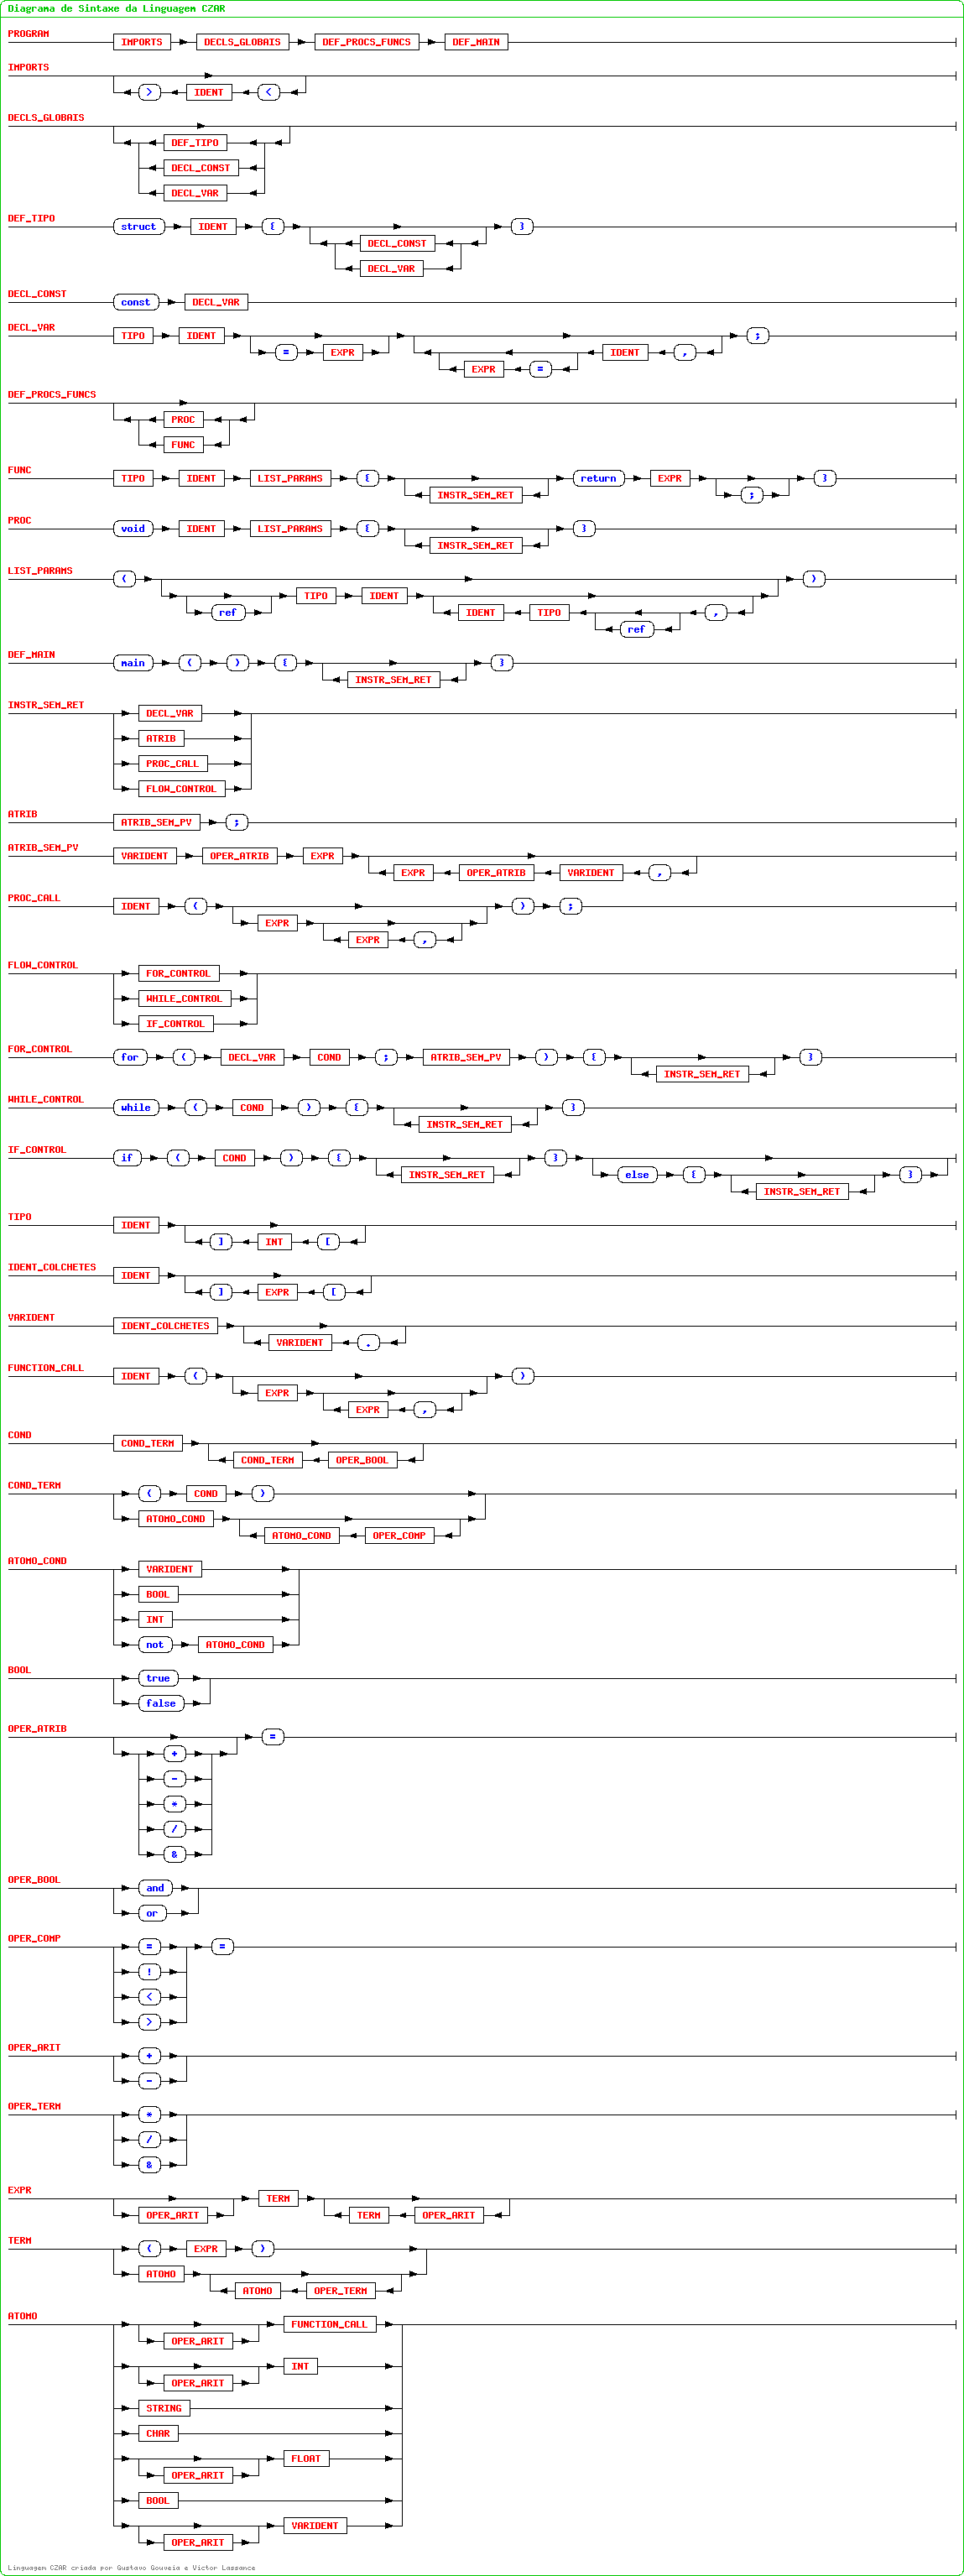
\includegraphics[width=\textwidth, clip, trim=0 1635px 0 0]{images/diagrama-sintaxe.png}  
	\label{fig:diagrama-sintaxe-1}
\end{figure}

\begin{figure}
	\centering 
	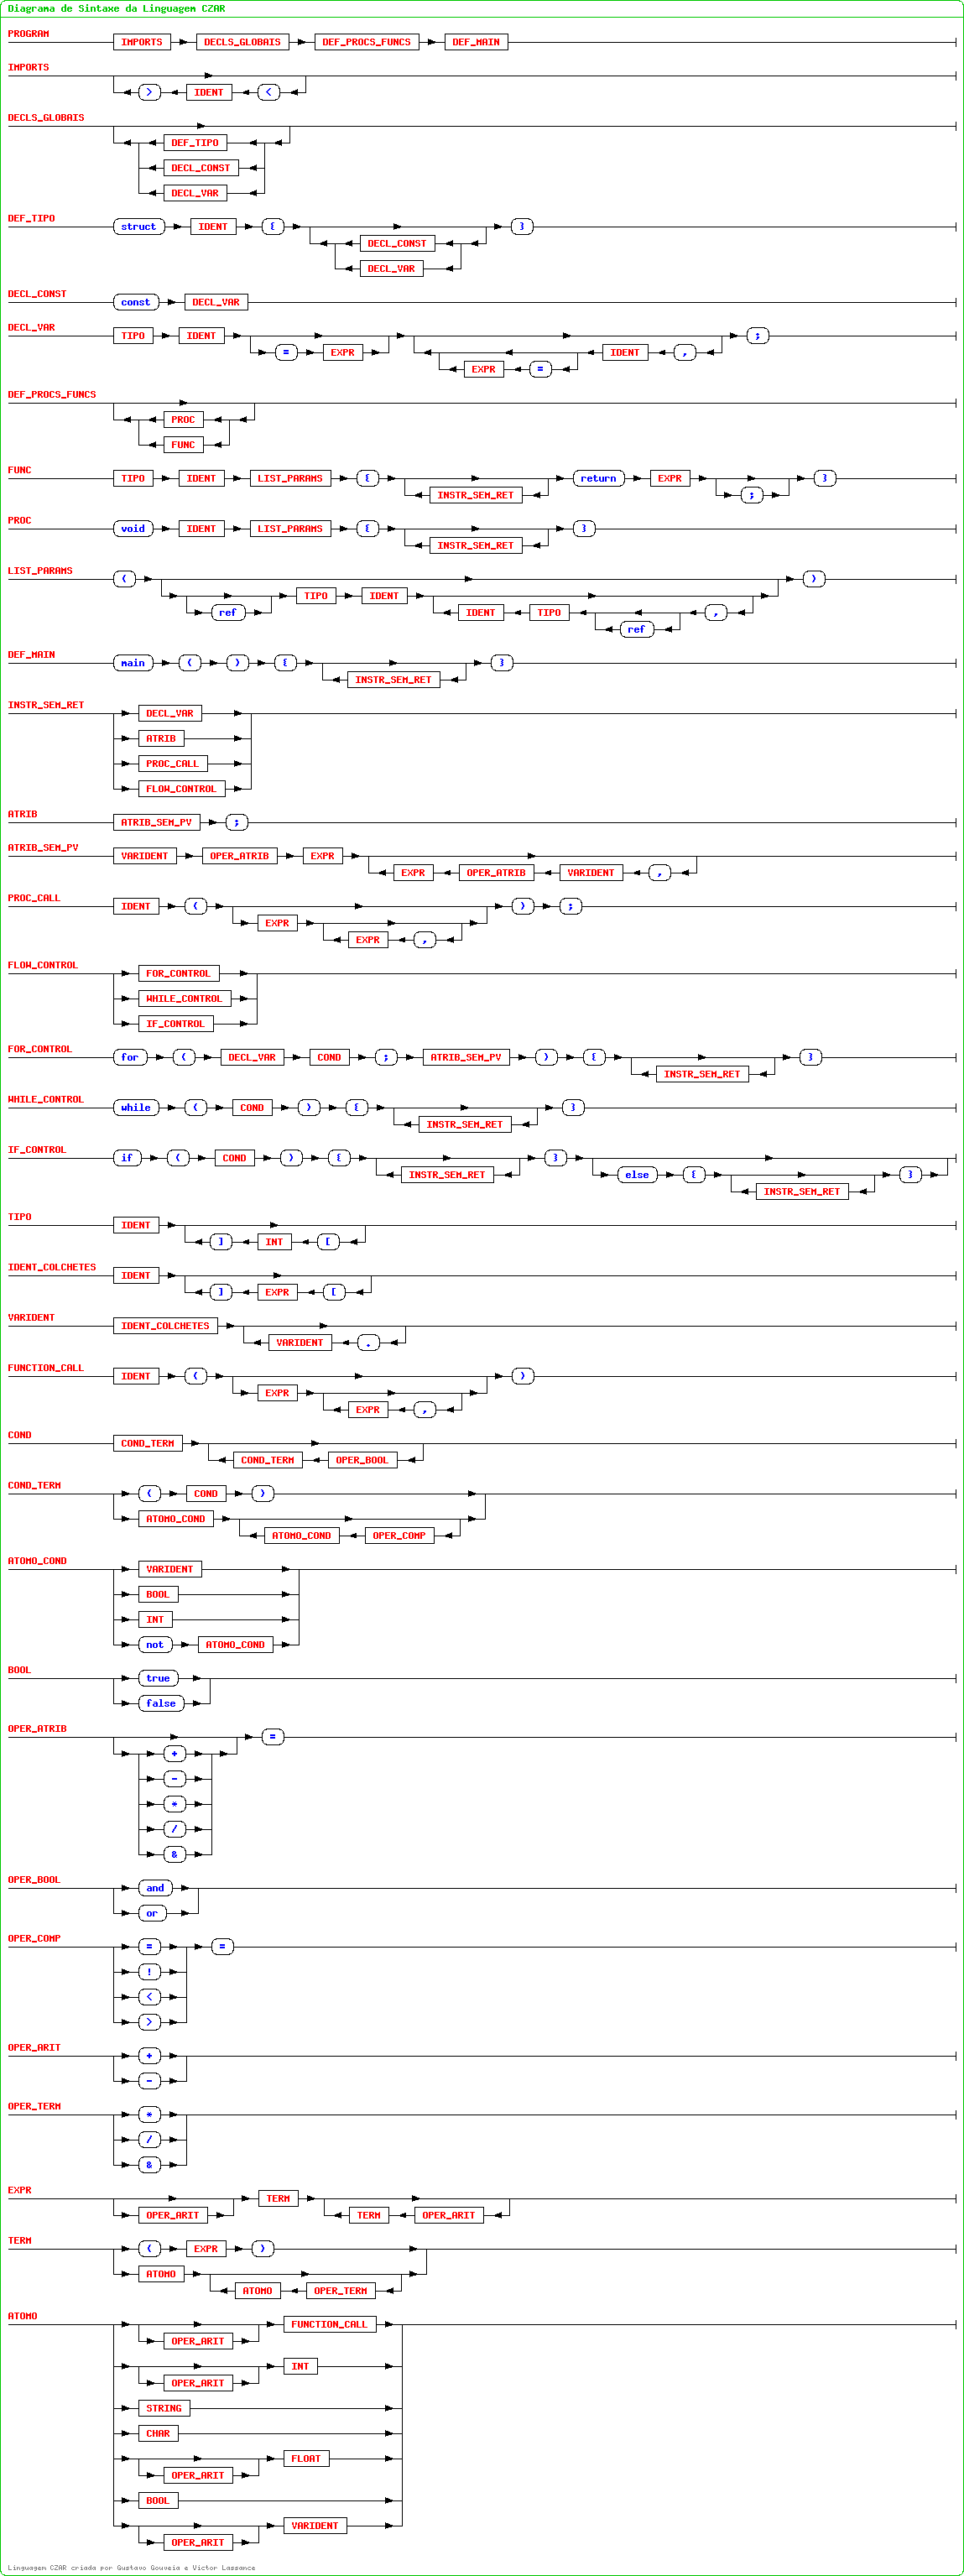
\includegraphics[width=\textwidth, clip, trim=0 0 0 1435px]{images/diagrama-sintaxe.png} 
	\caption{Diagrama de Sintaxe da Linguagem CZAR}
	\label{fig:diagrama-sintaxe-2}
\end{figure}


\chapter{Descrição do analisador léxico}
\label{chap:lexico}
	% !TEX encoding = UTF-8 Unicode

Em um primeiro momento, foi definida uma linguagem de programação e identificados os tipos de átomos. Para cada átomo foi escrito uma gramática linear representativa da sua lei de formação e um reconhecedor para o átomo. Desse modo, as gramáticas assim escritas foram unidas e convertidas em um autômato finito, o qual foi transformado em um transdutor e implementado como sub-rotina, dando origem ao analisador léxico propriamente dito.

Também foi criada uma função principal para chamar o analisador léxico e possibilitar o seu teste. Cabe ressaltar que foi utilizado o analisador léxico do trabalho como base para esse, visto que a estrutura e alguns \emph{tokens} eram os mesmos. Algumas das alterações feitas para adaptar o transdutor foram:

\begin{itemize}
	\item \textbf{IDENT vs PRED + INF}: Antes, só havíamos um \emph{token} para representar identificadores de alguma forma, chamados de \textbf{IDENT}. Porém, ao observar a sintaxe do \emph{SimpPro}, foi necessário alterar o léxico para diferenciar tokens que começam com minúscula (chamado \textbf{PRED}) ou maiúscula (chamado \textbf{INF});
	\item Os operadores específicos dessa linguagem como :- e ?- foram considerados novas classes de \emph{tokens}, para facilitar a sua identificação.
\end{itemize} 

A Figura~\ref{fig:transdutor} representa o transdutor utilizado para reconhecer os \emph{tokens} da linguagem.

\begin{figure}[htbp]
    \centering
    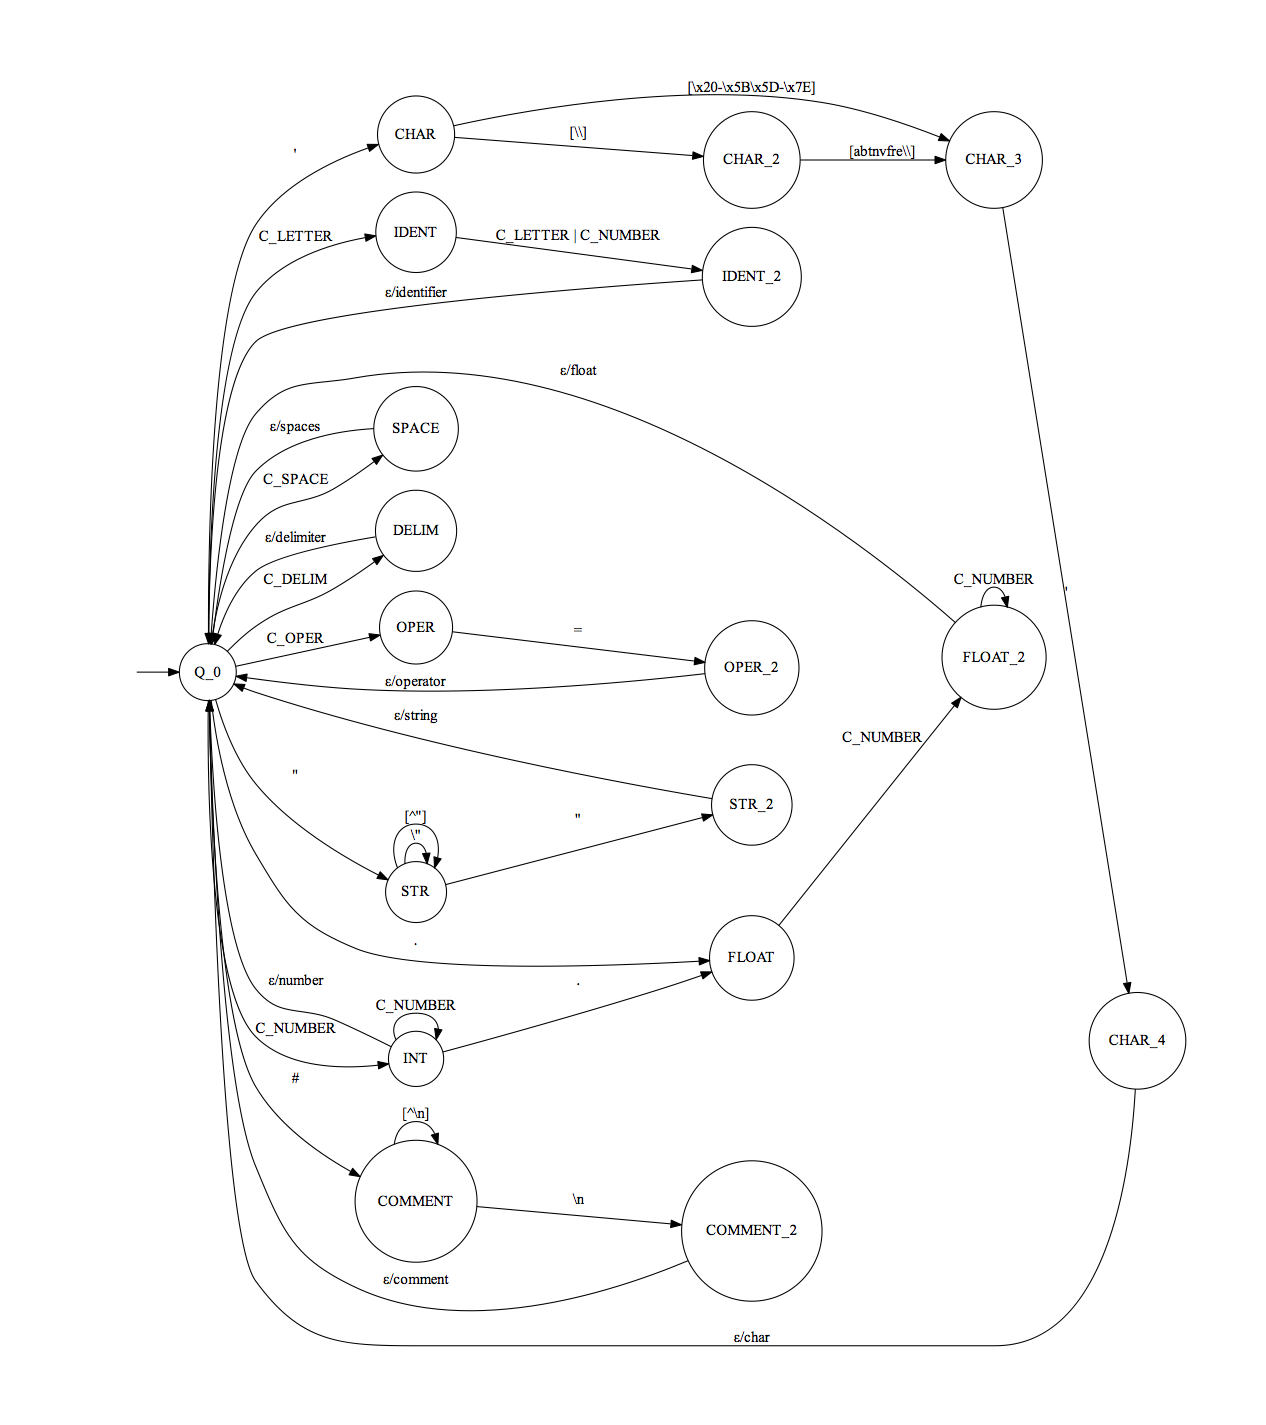
\includegraphics[width=0.7\textwidth]{./images/transdutor.png}
    \caption{Transdutor desenvolvido}
    \label{fig:transdutor}
\end{figure}


\chapter{Descrição do reconhecedor sintático}
\label{chap:sintatico}
	% !TEX encoding = UTF-8 Unicode

A criação do analisador sintático, assim como com o analisador léxico, ocorreu antes da segunda prova e utilizou parte da estrutura criada para o trabalho da disciplina.

A título de recordação, o papel do analisador sintático é obter uma cadeia de tokens proveniente do analisador léxico, e verificar se a mesma pode ser gerada pela gramática da linguagem e, com isso, construir a árvore sintática. Com isso em mente, convertemos a sintaxe da linguagem \emph{SimpPro} para WIRTH, como visto abaixo.

\lstinputlisting[frame=single,breaklines=true,numbers=left]{files/WIRTHorig.txt}

A partir do WIRTH acima, reduzimos a sintaxe para conter somente um autômato, como mostrado abaixo.

\lstinputlisting[frame=single,breaklines=true,numbers=left]{files/WIRTH.txt}

Através de um script, o WIRTH gerado foi então submetido ao site do Hugo Baraúna, seu resultado salvo em arquivos locais, o JFLAP aberto automaticamente e a figura do autômato armazenada localmente, além de gerar automaticamente o pdf impresso para a primeira parte da segunda prova. A Figura~\ref{fig:automato} mostra o autômato final.

\begin{figure}[htbp]
    \centering
    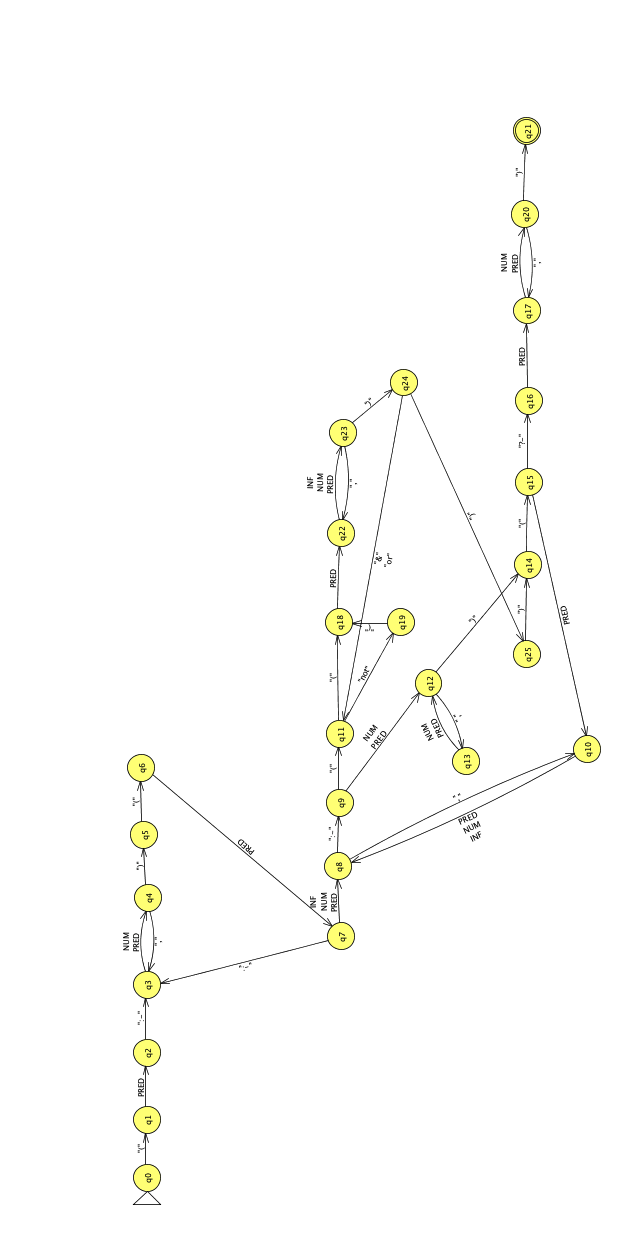
\includegraphics[width=0.75\textwidth]{./images/automato.png}
    \caption{Autômato \emph{Program}}
    \label{fig:automato}
\end{figure}

	
\chapter{Linguagem de montagem}
\label{chap:linguagem-montagem}
	% !TEX encoding = UTF-8 Unicode

O compilador por nós criado terá como linguagem de saída um programa que será executado na máquina virtual chamada Máquina de von Neumann (MVN).

O Modelo de von Neumann procura oferecer uma alternativa prática, disponibilizando ações mais poderosas e ágeis em seu repertório de operações que o modelo de Turing. Isso viabiliza, codificações muito mais expressivas, compactas e eficientes. Para isso, a Máquina de von Neumann utiliza:

\begin{itemize}
	\item Memória endereçável, usando acesso aleatório
	\item Programa armazenado na memória, para definir diretamente a função corrente da máquina (ao invés da Máquina de Estados Finitos)
	\item Dados representados na memória (ao invés da fita)
	\item Codificação numérica binária em lugar da unária
	\item Instruções variadas e expressivas para a realização de operações básicas muito frequentes (ao invés de sub-máquinas específicas)
	\item Maior flexibilidade para o usuário, permitindo operações de entrada e saída, comunicação física com o mundo real e controle dos modos de operação da máquina 
\end{itemize}

Dessa forma, utilizaremos essa máquina para executar nosso compilador e realizar os testes necessários.

\begin{figure}[ht]
	\centering
	\caption{Arquitetura MVN}
	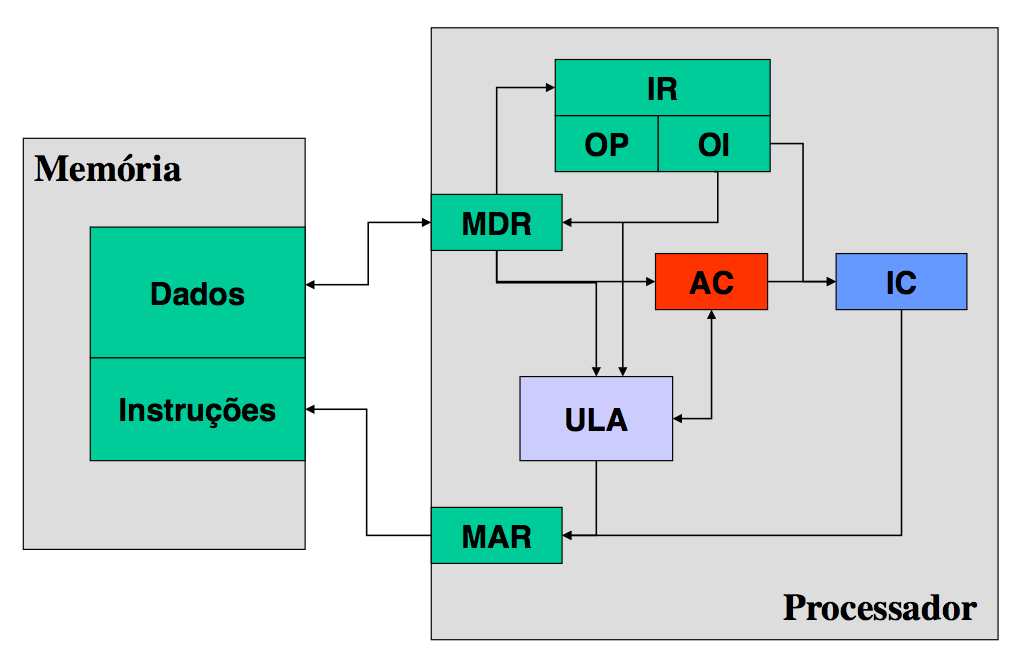
\includegraphics[width=\textwidth]{images/arquitetura-mvn.png}
	\label{fig:arquitetura-mvn}
\end{figure}

A arquitetura de Von Neumann é composta por um processador e uma memória principal. Na memória principal armazenam-se as instruções do código-fonte e os dados, sendo a divisão mostrada na figura~\ref{fig:arquitetura-mvn} apenas ilustrativa. Além da Unidade Lógica Aritmética (ULA), responsável pelo processamento de operações lógicas e aritméticas, o processador possui um conjunto de elementos físicos de armazenamento de informações e é comum dividir esses componentes nos seguintes módulos resgistradores:

\begin{enumerate}
	\item MAR - Registrador de endereço de memória
	
	Indica qual é a origem ou o destino, na memória principal, dos dados contidos no registrador de dados de memória.
	
	\item MDR -  Registrador de dados da memória
	
	Serve como ponte para os dados que trafegam entre a memória e os outros elementos da máquina.

	\item IC - Registrador de endereço de instrução 

	Indica a cada instante qual será a próxima instrução a ser executada pelo processador.

	\item IR -  Registrador de instrução

	Contém a instrução atual a ser executada. é subdividido em dois outros registradores, como na figura~\ref{fig:estrutura-ir}.
	\begin{figure}[ht]
		\centering
		\caption{Estrutura do registro de instrução (IR)}
		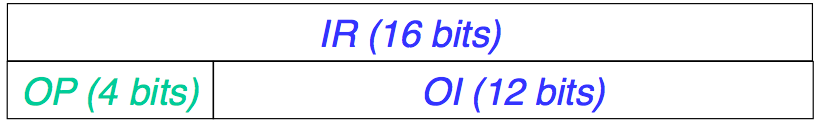
\includegraphics[width=0.8\textwidth]{images/estrutura-ir.png}
		\label{fig:estrutura-ir}
	\end{figure}

	\begin{enumerate}
		\item OP - Registrador de código de operação

		Parte do registrador de instrução que identifica a instrução que está sendo executada.

		\item OI - Registrador de operando de instrução

		Complementa a instrução indicando o dado ou o endereço sobre o qual ela deve agir.
	\end{enumerate}

	\item AC - Acumulador 

	Funciona como a área de trabalho para execução de operações lógicas ou aritméticas. Acumula o resultado de tais operações.
\end{enumerate}

A máquina executa um programa em diversos passos, listadas abaixo:

\begin{enumerate}
	\item Determinação da Próxima Instrução a Executar
	\item Fase de Obtenção da Instrução

	Obter na memória, no endereço contido no registrador de Endereço da Próxima Instrução, o código da instrução desejada.
	
	\item Fase de Decodificação da Instrução
	\label{item:decod-instrucao}

	Decompor a instrução em duas partes: o código da instrução e o seu operando, depositando essas partes nos registradores de instrução e de operando, respectivamente. Selecionar, com base no conteúdo do registrador de instrução, um procedimento de execução dentre os disponíveis no repertório do simulador (passo~\ref{item:exec-instrucao}).

	\item Fase de Execução da Instrução
	\label{item:exec-instrucao}
	
	Executar o procedimento selecionado no passo~\ref{item:decod-instrucao}, usando como operando o conteúdo do registrador de operando, preenchido anteriormente.
	
	Caso a instrução executada não seja de desvio, incrementar o registrador de endereço da próxima instrução a executar. Caso contrário, o procedimento de execução já terá atualizado convenientemente tal informação.
	
	\begin{enumerate}
		\item Execução da instrução (decodificada no passo~\ref{item:decod-instrucao})

		De acordo com o código da instrução a executar (contido no registrador de instrução), executar os procedimentos de simulação correspondentes (detalhados adiante).
		
		\item Acerto do registrador de Endereço da Próxima Instrução para apontar a próxima instrução a ser simulada:

		Incrementar o registrador de Endereço da Próxima Instrução.
	\end{enumerate}
	
\end{enumerate}


\section{Instruções da Linguagem de Saída}

As instruções da MVN podem ser resumidas pela tabela da figura~\ref{fig:instrucoes-mvn}.

\begin{figure}[ht]
	\centering
	\caption{Lista de instruções da MVN}
	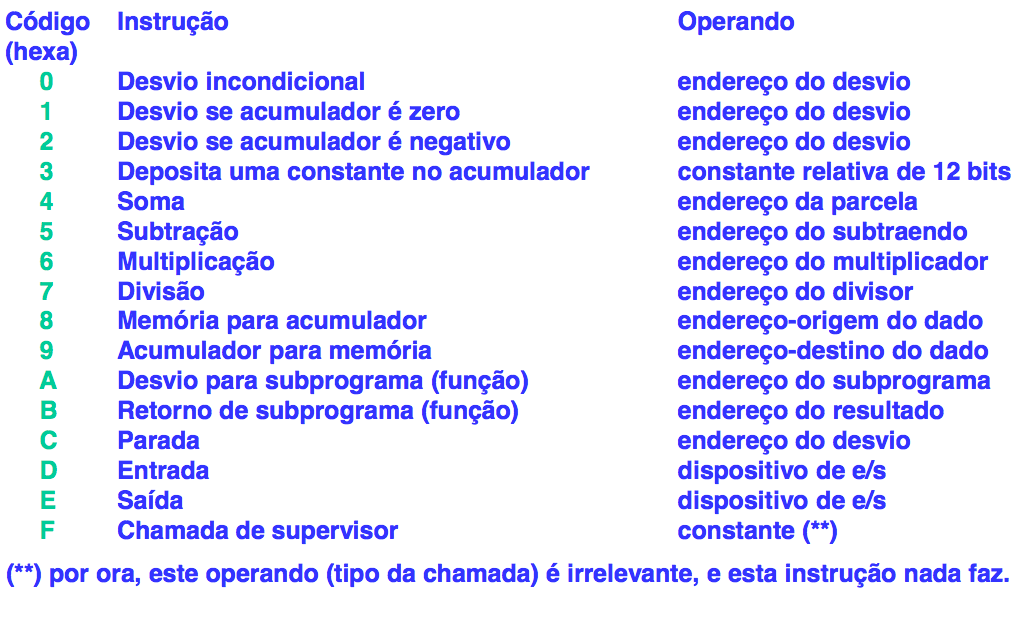
\includegraphics[width=\textwidth]{images/instrucoes-mvn.png}
	\label{fig:instrucoes-mvn}
\end{figure}

A seguir, especificaremos o que é realizado pela máquina ao executar cada tipo de operação.		

\begin{itemize}
	\item Registrador de instrução = 0 (desvio incondicional)

	Modifica o conteúdo do registrador de Endereço da Próxima Instrução (IC) armazenando nele o conteúdo do registrador de operando (OI)

	IC := OI

	\item Registrador de instrução = 1 (desvio se acumulador é zero)

	Se o conteúdo do acumulador (AC) for zero, então modifica o conteúdo do registrador de Endereço da Próxima Instrução (IC), armazenando nele o conteúdo do registrador de operando (OI) 

	Se AC = 0 então IC := OI 
	
	Se não IC := IC + 1 

	\item Registrador de instrução = 2 (desvio se negativo)

	Se o conteúdo do acumulador (AC) for negativo, isto é, se o bit mais significativo for 1, então modifica o conteúdo do registrador de Endereço da Próxima Instrução (IC) armazenando nele o conteúdo do registrador de operando (OI)

	Se AC < 0 então IC := OI 
	
	Se não IC := IC + 1

	\item Registrador de instrução = 3 (constante para acumulador)

	Armazena no acumulador (AC) o número relativo de 12 bits contido no registrador de operando (OI), estendendo seu bit mais significativo (bit de sinal) para completar os 16 bits do acumulador
		
	AC := OI 
	
	IC := IC +1 

	\item Registrador de instrução = 4 (soma)

	Soma ao conteúdo do acumulador (AC) o conteúdo da posição de memória indicada pelo registrador de operando MEM[OI]. Guarda o resultado no acumulador

	AC := AC + MEM[OI] 

	IC := IC + 1

	\item Registrador de instrução = 5 (subtração)

	Subtrai do conteúdo do acumulador (AC) o conteúdo da posição de memória indicada pelo registrador de operando MEM[OI]. Guarda o resultado no acumulador

	AC := AC - MEM[OI]

	IC := IC + 1 
		
	\item Registrador de instrução = 6 (multiplicação)

	Multiplica o conteúdo do acumulador (AC) pelo conteúdo da posição de memória indicada pelo registrador de operando MEM[OI]. Guarda o resultado no acumulador

	AC := AC * MEM[OI] 

	IC := IC + 1

	\item Registrador de instrução = 7 (divisão inteira)

	Dividir o conteúdo do acumulador (AC) pelo conteúdo da posição de memória indicada pelo registrador de operando MEM[OI]. Guarda a parte inteira do resultado no acumulador

	AC := int (AC / MEM[OI])

	IC := IC + 1 
			
	\item Registrador de instrução = 8 (memória para acumulador)

	Armazena no acumulador (AC) o conteúdo da posição de memória endereçada pelom registrador de operando (OI) 

	AC := MEM[OI]		

	IC := IC + 1
			
	\item Registrador de instrução = 9 (acumulador para memória)

	Guarda o conteúdo do acumulador (AC) na posição de memória endereçada pelo registrador de operando (OI) 

	MEM[OI] := AC		
	
	IC := IC + 1 
			
	\item Registrador de instrução = A (desvio para subprograma)

	Armazena o conteúdo do registrador de Endereço da Próxima Instrução (IC), incrementado de uma unidade, no registrador de endereço de retorno (RA). Armazena no registrador de Endereço da Próxima Instrução (IC) o conteúdo do registrador de operando (OI).

	RA := IC + 1
	
	IC := OI

	\item Registrador de instrução = B (retorno de subprograma)

	Armazena no registrador de Endereço da Próxima Instrução (IC) o conteúdo do registrador de endereço de retorno (RA), e no acumulador (AC) o conteúdo da posição de memória apontada pelo registrador de operando (OI) 

	AC := MEM[OI]			

	IC := RA 	 	 	 		

			
	\item Registrador de instrução = C (stop)

	Modifica o conteúdo do registrador de Endereço da Próxima Instrução (IC) armazenando nele o conteúdo do registrador de operando (OI) e para o processamento

	IC := OI

	\item Registrador de instrução = D (input)
 					
	Aciona o dispositivo padrão de entrada e aguardar que o usuário forneça o próximo dado a ser lido. Transfere o dado para o acumulador 

	Aguarda
	
	AC := dado de entrada 
	
	IC := IC + 1 
		
	\item Registrador de instrução = E (output)

	Transfere o conteúdo do acumulador (AC) para o dispositivo padrão de saída. Aciona o dispositivo padrão de saída e aguardar que este termine de executar a operação de saída 

	dado de saída := AC 

	aguarda
	
	IC := IC + 1

	\item Registrador de instrução = F (supervisor call)

	Não implementado: por enquanto esta instrução não faz nada.

	IC := IC + 1
\end{itemize}

Escrever um programa usando diretamente codificação binária não é uma tarefa simples, e tampouco agradável. Naturalmente, se um programa é muito grande ou se lida com diversas estruturas complexas (listas, etc.), a sua codificação se torna ainda mais difícil e complexa.

Por conta disso, torna-se imprescindível construir alguma abstração que facilite a programação e a verificação dos programas. A primeira idéia, mais natural, é utilizar o modelo de máquina existente e, a partir dele, definir nomes (mnemônicos) para cada instrução da máquina. Posteriormente, verifica-se que somente isso não basta, pois é necessário lidar com os endereços dentro de um programa (rótulos, operandos, sub-rotinas), com a reserva de espaço para tabelas, com valores constantes. Enfim, é necessário definir uma linguagem simbólica.

\begin{figure}[ht]
	\centering
	\caption{Esquema geral de um montador}
	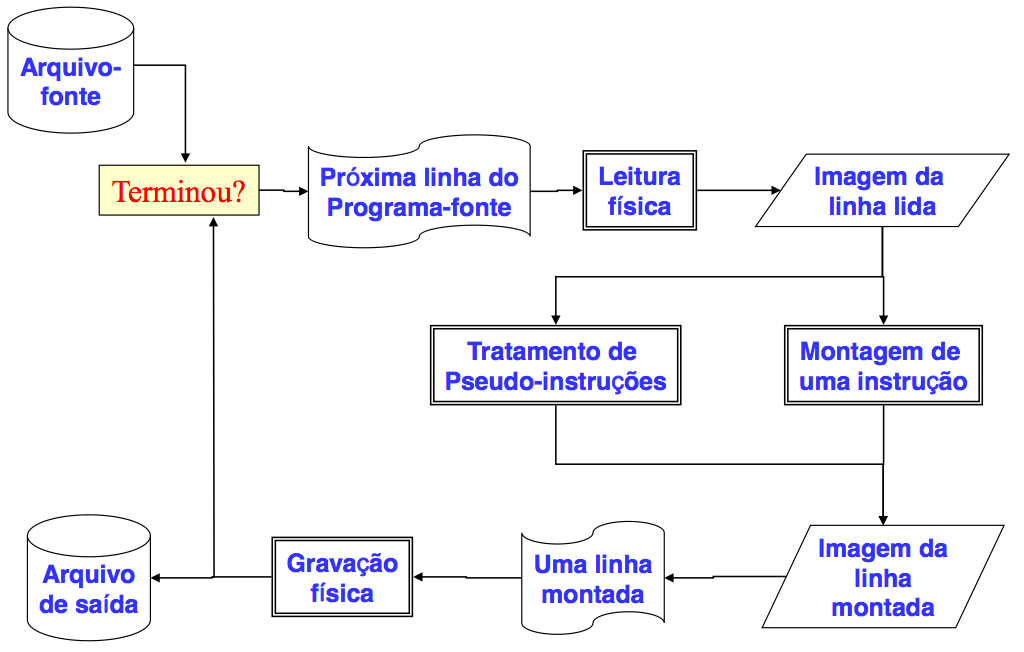
\includegraphics[width=\textwidth]{images/esquema-montador.png}
	\label{fig:esquema-montador}
\end{figure}

Para a construção de um montador, cujo esquema geral está representado na figura~\ref{fig:esquema-montador} pressupõe-se que sejam tratadas as seguintes questões:

\begin{itemize}
	\item definição das instruções: determinar os mnemônicos que as representam simbolicamente;
	\item definição das pseudo-instruções: determinar os mnemônicos que as representam, bem como sua função para o montador.
\end{itemize}

As instruções para a MVN são apresentadas na figura~\ref{fig:mnemonicos-mvn}.

\begin{figure}[ht]
	\centering
	\caption{Tabela de mnemônicos para a MVN (de 2 caracteres)}
	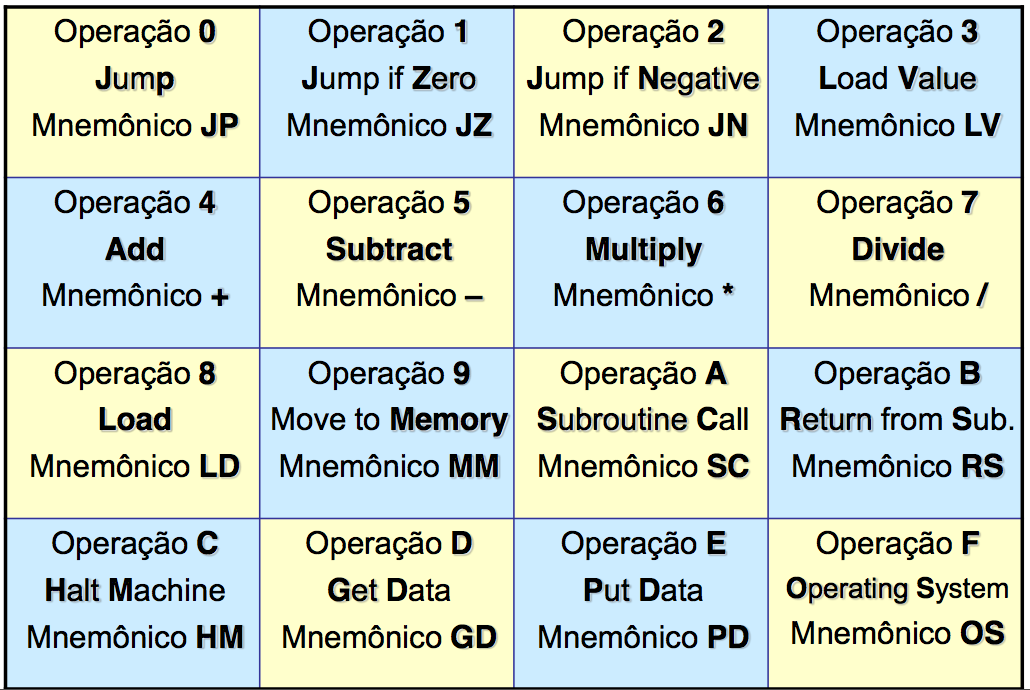
\includegraphics[width=\textwidth]{images/mnemonicos-mvn.png}
	\label{fig:mnemonicos-mvn}
\end{figure}


\section{Pseudoinstruções da Linguagem de Saída}

Programas absolutos são executáveis estritamente nas posições de memória em que foram criados, tornando difícil a manutenção e o trabalho em equipe. A utilização de programas relocáveis permitem sua execução em qualquer posição de memória, tornando possível utilizar partes de código projetadas externamente (uso de bibliotecas, por exemplo).

Para que se possa exprimir um programa relocável e com possibilidade de construção em módulos, separadamente desenvolvidos, é necessário que:
\begin{itemize}
	\item Haja a possibilidade de representar e identificar endereços absolutos e endereços relativos;
	\item Um programa possa ser montado sem que os seus endereços simbólicos estejam todos resolvidos;
	\item Seja possível identificar, em um módulo, símbolos que possam ser referenciados simbolicamente em outros módulos.
\end{itemize}

Sendo assim, a linguagem simbólica não possui somente os mnemônicos das instruções da MVN, mas também comandos chamados de pseudo-instruções da linguagem de montagem. Na linguagem de montagem, as pseudo-instruções também são representadas por mnemônicos, listados abaixo:

\begin{itemize}
	\item @ : Origem Absoluta. Recebe um operando numérico, define o endereço da instrução seguinte;
	\item K : Constante, o operando numérico tem o valor da constante (em hexadecimal). Define uma área preenchida por uma CONSTANTE de 2 bytes;
	\item \$ : Reserva de área de dados, o operando numérico define o tamanho da área a ser reservada. Define um BLOCO DE MEMóRIA com número especificado de words;
	\item \# : Final físico do texto fonte;
	\item \& : Origem relocável;
	\item > : Endereço simbólico de entrada (entry point). Define um endereço simbólico local como entry-point do programa;
	\item < : Endereço simbólico externo (external). Define um endereço simbólico que referencia um entry-point externo.
\end{itemize}

Na figura~\ref{fig:exemplo-somador}, temos um exemplo de um somador escrito em linguagem de montagem, visto na aula de Fundamentos de Eng. de Computação, e sua respectiva tradução pelos módulos Montador, \emph{Linker} e Relocador, módulos extras porém integrados no nosso caso:

\begin{figure}[ht]
	\centering
	\caption{Exemplo de um somador}
	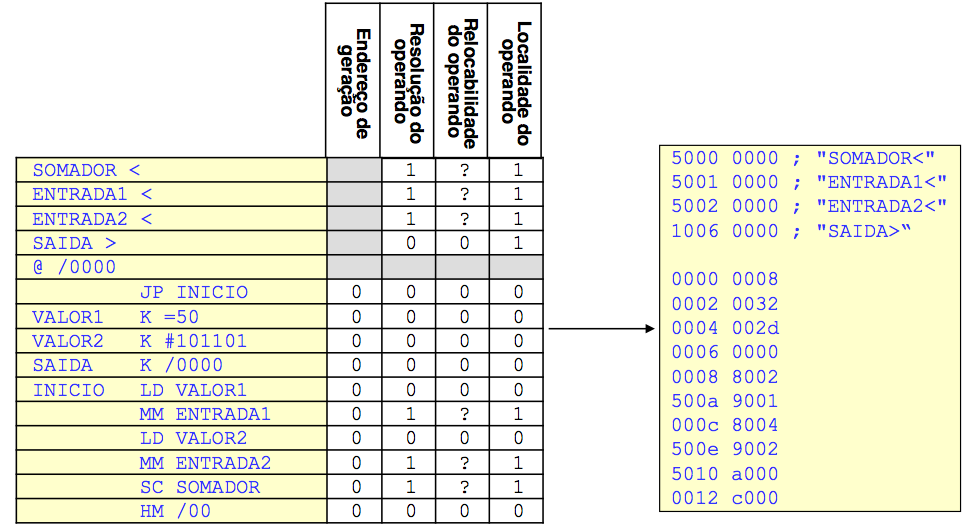
\includegraphics[width=\textwidth]{images/exemplo-somador.png}
	\label{fig:exemplo-somador}
\end{figure}



\chapter{Ambiente de execução}
\label{chap:ambiente-execucao}
	% !TEX encoding = UTF-8 Unicode

\section{Características gerais}

\subsection{Organização da memória}

O ambiente de execução da MVN fornece aos programadores um tamanho limitado de memória para ser usado no geral, a ser compartilhado entre o código e as variáveis do programa. O montador aloca a memória com base nos endereços relativos especificados no código do programa. Do total, a parte inicial da memória é reservada para guardar as instruções que serão executadas pelo programa. A parte final da memória deve ser usada especialmente para o uso do registro de ativação.

De maneira mais objetiva, reserva-se uma parte do código para a área de dados, uma parte para a função principal e as subrotinas e uma parte dedicada a pilhas de variáveis e endereços que viabilizam a chamada de subrotinas.

\subsection{Registro de ativação}

As funções em programas têm variáveis locais, que devem ser criadas na chamada da função e sobrevivem até que a função retorne. Elas também possuem recursão, onde cada instância da função tem seus próprios parâmetros e locais. As chamadas de funções se comportam de maneira LIFO, portanto podemos usar uma pilha como estrutura.

As operações push e pop dessa pilha não podem ser feitas individualmente para cada variável. Desa forma, manipula-se conjuntos de variáveis, e precisamos ter acesso a todas elas. Com isso, definimos dois conceitos:

\begin{itemize}
	\item \emph{Stack Pointer} (SP):
	\begin{itemize}
		\item Todas as posições além do SP são lixo;
		\item Todas as anteriores estão alocadas.
	\end{itemize}
	
	\item \emph{Activation Record} ou \emph{Stack Frame}
	\begin{itemize}
		\item área na pilha reservada para os dados de uma função (parâmetros, locais, endereço de retorno, etc).
                \item esta parte da pilha foi fusionada à parte anterior,
                    facilitando o uso da pilha e diminuindo a quantidade de
                    dados na mesma. Esta decisão não afeta a implantação, uma
                    vez que no caso desta linguagem o compilador tem total
                    controle do tamanho das estruturas sendo utilizadas. 
	\end{itemize}
\end{itemize}

\begin{figure}[ht]
	\centering
	\caption{Esquema do Registro de Ativação}
	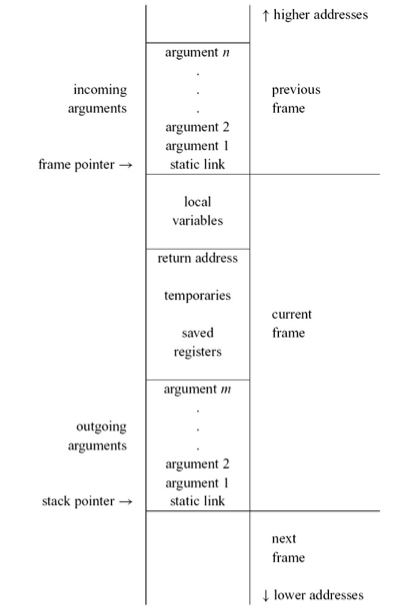
\includegraphics[width=0.5\textwidth]{images/registros-ativacao.png}
	\label{fig:registros-ativacao}
\end{figure}

A figura~\ref{fig:registros-ativacao} ilustra a organização da pilha. O uso do registro de ativação permite entre outras coisas a chamada recursiva de funções, uma vez isso não é possível de forma nativa no ambiente da MVN. No caso da MVN, a pilha cresce para baixo e as subrotinas são executadas utilizando as seguintes instruções:

\begin{itemize}
	\item Desvio para subprograma - mnemônico SC (0xA): armazena o endereço de instrução seguinte (atual + 1) na posição de memória apontada pelo operando. Em seguida, desvia a execução para o endereço indicado pelo operando e acrescido de uma unidade.
	
	\item Retorno de subprograma - mnemônico RS (0xB): desvia a execução para o endereço indicado pelo valor guardado na posição de memória do operando.
\end{itemize}

Foi criada por nós uma biblioteca em assembly para implementar funções auxiliares de entrada e saída de dados, além da funcionalidade de empilhar, desempilhar e ter acesso a informações contidas na pilha discutida anteriormente. Essas funções são explicadas na próxima seção.

\section{Biblioteca desenvolvida em Assembly}

A biblioteca padrão desenvolvida é dividida em dois módulos o primeiro
implementa as funções básicas de empilhamento, sendo chamado de \verb!std.asm!.
O segundo módulo implementa as operações de input e output de dados, de nome 
\verb!stdio.asm!.

\subsection{STD}

A manipulação de pilhas é feita pela biblioteca padrão, sendo que deseja-se
seguir a estrutura abaixo definida, facilitando o uso e acesso das variáveis.
Vemos abaixo um exemplo do uso da biblioteca. Na linha 23 salvamos uma variável
recebida por parâmetro na pilha e na linha 30 recuperamos seu valor. 

Logo antes de retornar devemos executar a função \verb!POP_CALL! 
ela é responsável por
escrever o endereço de retorno na função em que estamos, assim aproveitando das
chamadas existentes na \verb!MVN! (funções devem ser \emph{stateless} para tanto). Percebe-se
que é possível executar a função recursivamente (linha 55 e 57). Para tanto é
necessário chamar a função \verb!PUSH_CALL! para que a mesma efetue o
empilhamento e escreva o endereço de retorno atual na pilha. 

\begin{lstlisting}[basicstyle=\footnotesize,numbers=left,breaklines=true,morekeywords={}]
;; VARIAVEIS GLOBAIS
;; comeco da pilha = FFF 
;; tamanho da pilha = 2FF 
;;   | ptr to old_stack_head  | \___ STACK_PTR
;;   |      savedregist       |   
;;   |         ...            |   
;;   |      local var         |  
;;   |         ...            |   
;;   |      temporaries       |  
;;   |      parameters        |   
;;   |         ...            |  
;;   |     ref parameters     |  ____ OLD STACK_PTR
;;   |      returnaddrs       | /     (STACK_PTR points here)

EXAMPLE_STACK_ARG    K  /0000
EXAMPLE_STACK        JP /000 
                     SC PRINT_STACK_ADDRS   ;; deve imprimir 0fff 
                     ;;; SALVAR ARGUMENTOS na pilha 
                     LV =0
                     MM WORD_TO_SAVE 
                     LV EXAMPLE_STACK_ARG 
                     MM ORIGIN_PTR 
                     SC SAVE_WORD_TO_LOCAL_VAR 
                     ;;;; CORPO DA FUNCAO 
                     ;;; CARREGANDO UM VALOR DA PILHA 
                     LV =0
                     MM WORD_TO_GET 
                     LV EXAMPLE_STACK_ARG 
                     MM STORE_PTR
                     SC GET_WORD_LOCAL_VAR 
                     ;;; IMPRIME 
                     LV COUNT_IS
                     MM STRING_PTR 
                     SC P_STRING  ;; inline fct, no need to stack 
                     LD EXAMPLE_STACK_ARG 
                     MM TO_BE_PRINTED 
                     SC P_INT_ZERO
                     SC P_LINE

                     LD EXAMPLE_STACK_ARG
                     JZ RETURN_EXAMPLE_STACK

                     LD EXAMPLE_STACK_ARG 
                     -  ONE 
                     MM EXAMPLE_STACK_ARG 

                     LV =1
                     MM PUSH_CALL_SIZELV
                     LV =0
                     MM PUSH_CALL_RET_ADDRS 
                     LV =0
                     MM PUSH_CALL_TMP_SZ
                     LV =0
                     MM PUSH_CALL_PAR_SZ 
                     SC PUSH_CALL

                     SC EXAMPLE_STACK  ;; chamada recursiva
                     ;;;; FIM DO CORPO DA FUNCAO 
RETURN_EXAMPLE_STACK LV EXAMPLE_STACK
                     MM POP_CALL_FCT 
                     SC POP_CALL ;; trickery!

                     SC PRINT_STACK_ADDRS   ;; deve imprimir 0fff 
                     RS EXAMPLE_STACK
\end{lstlisting}

Abaixo podemos ver a implementação das funções de \verb!PUSH! e \verb!POP!

A pilha é implementada dos valores mais altos da memória para os valores mais
baixos, sendo assim, o ponteiro de pilha começa apontando para \verb!0x0FFF!.

A pilha funciona como uma lista ligada que guarda o endereço da última célula
da pilha. Sendo assim, a operação de \verb!POP! é trivial. Estas funções fazem
a gestão do endereço de retorno automaticamente, contanto que se siga a
premissa de chamada (chamada da função logo após a chamada de \verb!PUSH_CALL!
e seus parâmetros).

\begin{lstlisting}[basicstyle=\footnotesize,numbers=left,breaklines=true,morekeywords={}]
;; *** PUSH_CALL ***
PUSH_CALL           JP /000 
                    LD PUSH_CALL  ;; get return addrs 
                    +  TWO ;; return address of the callee
                    +  LOADV_CONST
                    MM LOAD_RETURN_ADDRS 
                    LD STACK_PTR
                    -  TWO        ;; new return addrs  
                    +  MOVE_CONST 
                    MM MOVE_RETURN_ADDRS 
LOAD_RETURN_ADDRS   JP /000  
MOVE_RETURN_ADDRS   JP /000   ;; return addrs salvo 
                    LD STACK_PTR          
                    -  TWO 
                    -  TWO 
                    -  PUSH_CALL_SIZELV
                    -  PUSH_CALL_RET_ADDRS
                    -  PUSH_CALL_TMP_SZ
                    -  PUSH_CALL_PAR_SZ 
                    -  TWO  ;; return addrs
                    MM TMP_1
                    LD TMP_1 
                    +  MOVE_CONST 
                    MM MRKR_PC_SAVE_HEAD 
                    LD STACK_PTR 
MRKR_PC_SAVE_HEAD   JP /000 
                    LD TMP_1 
                    MM STACK_PTR
                    RS PUSH_CALL
;; **** POP_CALL ****

POP_CALL_FCT        K /0000             
POP_CALL            JP /000 ; retorno 
POP_CALL_INIT       LD STACK_PTR 
                    +  LOAD_CONST 
                    MM MRKR_PC_LOAD_HEAD 
MRKR_PC_LOAD_HEAD   JP /000 
                    MM STACK_PTR 
                    LD STACK_PTR 
                    -  TWO
                    +  LOAD_CONST 
                    MM LOAD_RETURN_ADDRS_2
                    LD POP_CALL_FCT 
                    +  MOVE_CONST 
                    MM MOVE_RETURN_ADDRS_2
LOAD_RETURN_ADDRS_2 JP /000 
MOVE_RETURN_ADDRS_2 JP /000  ;; engana a funcao para ela pensar que ela 
                             ;; tem que retornar para esse valor 
                    RS POP_CALL
\end{lstlisting}


As rotinas de salvaguarda e carregamento dos valores locais, parâmetros,
   referências pode ser feita por meio das chamadas abaixo, 
   \verb!SAVE_WORD_TO_LOCAL_VAR! e \verb!GET_WORD_LOCAL_VAR! respectivamente.

\begin{lstlisting}[basicstyle=\footnotesize,numbers=left,breaklines=true,morekeywords={}]
;; **** SAVE_WORD_TO_LOCAL_VAR WORD_TO_SAVE ORIGIN_PTR ****
SAVE_WORD_TO_LOCAL_VAR      JP /000 
                            LD STACK_PTR
                            + TWO          ;; first word 
                            + WORD_TO_SAVE 
                            + WORD_TO_SAVE  ;; WORD_TO_GET * 2
                            + MOVE_CONST   ;; 
                            MM MOVE_WORD_LOCAL_VAR_2
                            LD ORIGIN_PTR
                            + LOAD_CONST 
                            MM LOAD_WORD_LOCAL_VAR_2
LOAD_WORD_LOCAL_VAR_2       JP /000 ;; 8FROMPTR
MOVE_WORD_LOCAL_VAR_2       JP /000 ;; 9TOPTR
                            RS SAVE_WORD_TO_LOCAL_VAR

;; **** GET_WORD_LOCAL_VAR WORD_TO_GET STORE_PTR ****


WORD_TO_GET        K /000 
STORE_PTR          K /000

GET_WORD_LOCAL_VAR          JP /000 
                            LD STACK_PTR
                            + TWO          ;; first word 
                            + WORD_TO_GET  
                            + WORD_TO_GET  ;; WORD_TO_GET * 2
                            + LOAD_CONST   ;; 
                            MM LOAD_WORD_LOCAL_VAR  
                            LD STORE_PTR
                            + MOVE_CONST 
                            MM MOVE_WORD_LOCAL_VAR
LOAD_WORD_LOCAL_VAR         JP /000 ;; 8FROMPTR
MOVE_WORD_LOCAL_VAR         JP /000 ;; 9TOPTR
                            RS GET_WORD_LOCAL_VAR
 \end{lstlisting}


\subsection{STDIO}


O ambiente de execução também é provido de funções de input/output:

Para a impressão de \emph{strings} podemos utilizar a função \verb!P_STRING!, 
     passando o ponteiro para o começo de uma \verb!string!. Em \verb!CZAR!
     consideramos \emph{strings} como sendo \emph{bytes} em um vetor de
     \emph{word} terminados pelo \emph{byte} \verb!0x0000!. Vale salientar que
     esta forma de armazenamento não causa problemas com outros tipos de
     armazenamento mais compactos, como a utilização dos dois \emph{bytes}
     da \emph{word} para armazenamento de \emph{chars} subsequentes. Quando a
     função recebe a \emph{word} \verb!0x0030!, primeiramente ela vai imprimir
     \verb!0x00! que é o caractere nulo, portanto, sem impressão e então
     imprimir o caractere correspondente a \verb!0x30!. 

\begin{lstlisting}[basicstyle=\footnotesize,numbers=left,breaklines=true,morekeywords={}]
;; ****  P_STRING &STRING_PTR ****
;;   Imprime a string apontada por STRING_PTR ate
;; o caractere /000  

P_STRING            JP /000           ; endereco de retorno 
PSTRINGINIT         LD STRING_PTR 
                    MM TO_BE_PRINTED_TMP 
LOAD_TO_BE_PRINTED  LD TO_BE_PRINTED_TMP
                    +  LOAD_CONST    
                    MM LABELLOAD 
LABELLOAD           K  /0000 
                    JZ P_STRING_END  ; se zero vamos para o final!
                    PD /100 
                    LD TO_BE_PRINTED_TMP
                    +  TWO
                    MM TO_BE_PRINTED_TMP
                    JP LOAD_TO_BE_PRINTED
P_STRING_END        RS P_STRING 

 \end{lstlisting}

Para a leitura de \emph{strings} seguimos o padrão definido anteriormente, um
\emph{byte} (\emph{char}) por \emph{word}:

\begin{lstlisting}[basicstyle=\footnotesize,numbers=left,breaklines=true,morekeywords={}]
;; *** GETS STORE_PTR_IO ***
;; Existe um problema de buffer aqui... nao vamos 
;; trata-lo, pois este e' um problema intri'nseco da 
;; MVN. (leitura e subsequente bloqueio por word)
LAST_CONTROL_CHAR_P_ONE    K /0021
ARRAY_POS_BYTE  JP /000
GETS            JP /000
                LD STORE_PTR_IO
                MM ARRAY_POS_BYTE
GETS_LOOP       GD /000
                MM HIGH_V
                SC HIGH_LOW 
                LD HIGH_V 
                -  LAST_CONTROL_CHAR_P_ONE 
                JN RETURN_GETS 
                LD ARRAY_POS_BYTE 
                +  MOVE_CONST 
                MM MOVE_HIGH_V
                LD HIGH_V 
MOVE_HIGH_V     JP /000 

                LD ARRAY_POS_BYTE
                +  TWO 
                MM ARRAY_POS_BYTE 

                LD LOW_V 
                -  LAST_CONTROL_CHAR_P_ONE 
                JN RETURN_GETS 
                LD ARRAY_POS_BYTE 
                +  MOVE_CONST 
                MM MOVE_LOW_V
                LD LOW_V 
MOVE_LOW_V      JP /000 

                LD ARRAY_POS_BYTE
                +  TWO 
                MM ARRAY_POS_BYTE 

                JP GETS_LOOP 

RETURN_GETS     LD ARRAY_POS_BYTE 
                +  MOVE_CONST 
                MM MOVE_ZERO
                LV =000  
MOVE_ZERO       JP /000 

                LD ARRAY_POS_BYTE
                +  TWO 
                MM ARRAY_POS_BYTE 
                RS GETS

\end{lstlisting}

A biblioteca também é capaz de realizar a leitura e escrita de valores
inteiros (funções auxiliares estão disponíveis no pacote em anexo): 

\begin{lstlisting}[basicstyle=\footnotesize,numbers=left,breaklines=true,morekeywords={}]
;; *** READ_INT STORE_PTR_IO ***
;; doesnt care about buffers, should have a trailing char at the end of the
;; stream otherwise it will just discard it.. 
STORE_PTR_IO        JP /000
ZERO_M_ONE          K  /002F
NINE_P_ONE          K  /0039

LOW                 K  /0000
HIGH                K  /0000
GO_IF_NUMBER        K  /0000 
TO_BE_TRIMMED       K  /0000 
TBT_TMP             K  /0000 

TRIM_INT            JP /000
                    LD TO_BE_TRIMMED
                    /  SHIFT_BYTE  
                    *  SHIFT_BYTE
                    MM TBT_TMP 
                    LD TO_BE_TRIMMED
                    -  TBT_TMP 
                    MM TO_BE_TRIMMED 
                    RS TRIM_INT 

READ_INT_WORD       JP /000
                    GD /000 
                    MM TMP_3 
                    LD TMP_3
                    /  SHIFT_BYTE
                    MM TO_BE_TRIMMED 
                    SC TRIM_INT 
                    LD TO_BE_TRIMMED
                    MM HIGH 

                    LD TMP_3
                    MM TO_BE_TRIMMED 
                    SC TRIM_INT
                    LD TO_BE_TRIMMED
                    MM LOW
                    RS READ_INT_WORD

READ_INT            JP /000 
                    LV =0 
                    MM TMP_4
READ_INT_LOOP       SC READ_INT_WORD 
                    LD HIGH 
                    MM TMP_3 
                    LV CONT1
                    MM GO_IF_NUMBER
                    JP IF_NUMBER_CONTINUE 
CONT1               LD LOW
                    MM TMP_3 
                    LV READ_INT_LOOP
                    MM GO_IF_NUMBER
                    JP IF_NUMBER_CONTINUE 
NOT_NUMBER          LD STORE_PTR_IO
                    +  MOVE_CONST 
                    MM MOVE_READ_INT
                    LD TMP_4 
MOVE_READ_INT       JP /000
                    RS READ_INT 

IF_NUMBER_CONTINUE  LD TMP_3 
                    -  ZERO_M_ONE 
                    JN NOT_NUMBER 
                    LD NINE_P_ONE 
                    -  TMP_3
                    JN NOT_NUMBER  

                    LD TMP_4
                    *  TEN 
                    MM TMP_4 


                    LD TMP_3 
                    -  ZERO_M_ONE
                    -  ONE 
                    +  TMP_4
                    MM TMP_4

                    LD GO_IF_NUMBER
                    MM END_READ_INT
END_READ_INT        JP /000
\end{lstlisting}

A impressão de inteiros, por ser crítica e muito importante para a correção de
erros, foi feita de forma simples e direta. Sem laços (unwind de \verb!GOTO!
    explícito) ou complicações,
    resultando em uma função bem determinada e robusta.
\begin{lstlisting}[basicstyle=\footnotesize,numbers=left,breaklines=true,morekeywords={}]
;; *** P_INT_ZERO TO_BE_PRINTED ***
;;  Imprime um inteiro (com zeros a esquerda)
;; ex:  
;;  INT_2 K  =345 
;;        LD INT_2
;;        MM TO_BE_PRINTED 
;;        SC P_INT_ZERO
;; imprime 00345
;;
;;
;; Esta funcao esta com o loop inline
;; sendo simples e robusta

P_INT_ZERO          JP /000
P_INT_INIT          JP P_INT_REAL_INIT
ZERO_BASE           K /30
;; bases para a conversao:
INT_POT_1           K =10000   
INT_POT_2           K =1000 
INT_POT_3           K =100  
INT_POT_4           K =10 
INT_POT_5           K =1 
P_INT_REAL_INIT     LD TO_BE_PRINTED       ;; PRIMEIRO CHAR
                    MM TMP_1 
                    /  INT_POT_1 
                    +  ZERO_BASE 
                    PD /100                     ;; imprime 
                    LD TMP_1  
                    /  INT_POT_1
                    *  INT_POT_1 
                    MM TMP_2                     
                    LD TMP_1
                    -  TMP_2
                    MM TMP_1   
                    /  INT_POT_2                ;; segundo char 
                    +  ZERO_BASE 
                    PD /100                     ;; imprime 
                    LD TMP_1  
                    /  INT_POT_2
                    *  INT_POT_2 
                    MM TMP_2                     
                    LD TMP_1
                    -  TMP_2
                    MM TMP_1 
                    /  INT_POT_3                ;; terceiro char 
                    +  ZERO_BASE 
                    PD /100                     ;; imprime 
                    LD TMP_1  
                    /  INT_POT_3
                    *  INT_POT_3 
                    MM TMP_2                     
                    LD TMP_1
                    -  TMP_2
                    MM TMP_1 
                    /  INT_POT_4                ;; quarto char 
                    +  ZERO_BASE 
                    PD /100                     ;; imprime 
                    LD TMP_1  
                    /  INT_POT_4
                    *  INT_POT_4 
                    MM TMP_2                     
                    LD TMP_1
                    -  TMP_2
                    MM TMP_1 
                    /  INT_POT_5                ;; quinto char 
                    +  ZERO_BASE 
                    PD /100                     ;; imprime 
                    LD TMP_1  
                    /  INT_POT_5
                    *  INT_POT_5 
                    MM TMP_2                     
                    LD TMP_1
                    -  TMP_2
                    MM TMP_1 
                    RS P_INT_ZERO

 \end{lstlisting}



\chapter{Tradução de comandos semânticos}
\label{chap:semantico}
	% !TEX encoding = UTF-8 Unicode

\section{Tradução de estruturas de controle de fluxo}

Será apresentado nas próximas seções, as traduções das estruturas de controle de fluxo que constam na nossa linguagem e foram solicitadas para essa entrega, entre elas as estruturas if, if-else e while.

Cabe ressaltar que foram utilizadas simbologias nas traduções que serão substituídas pelo compilador no momento da geração de código. Uma dessas marcações é os dois pontos no começo de uma linha que significa que os comandos devem ser colocados no início do código gerado. Outra simbologia criada é da forma {XN}, onde X representa uma letra maiúscula qualquer e N é o índice da instância dentro do tipo de marcação X. As opções para X são as seguintes:

\begin{itemize}
	\item \verb={C0}, {C1}, ...=: Conjunto de comandos
	\item \verb={R0}, {R1}, ...=: Referência
	\item \verb={L0}, {L1}, ...=: Label ou rótulo de uma instrução criados
            e exportados pelo código 
\end{itemize}

Há também a marcação \verb={N}=, utilizada para denotar que a primeira instrução do código subsequente ao comando atual deve ser adicionada no lugar da marcação. Estamos considerando substituir sempre a marcação \verb={N}= por uma instrução simples que só sirva para simplificar, como por exemplo somar zero ao acumulador.

Conceitos da pilha aritmética são utilizados para o cálculo de expressões
booleanas, no \autoref{sec:expre} explicações mais detalhadas são apresentadas. 

\subsection{Estrutura de controle de fluxo: IF}
\label{sec:if}

\lstinputlisting[frame=single,numbers=left,breaklines=true,morekeywords={JP,JZ,JN,LV,LD,MM,SC,RS,HM,GD,PD,OS}]{precompiled/if.pre}

\subsection{Estrutura de controle de fluxo: IF-ELSE}
\label{sec:if-else}

\lstinputlisting[frame=single,numbers=left,breaklines=true,morekeywords={JP,JZ,JN,LV,LD,MM,SC,RS,HM,GD,PD,OS}]{precompiled/ifelse.pre}

\subsection{Estrutura de controle de fluxo: WHILE}
\label{sec:while}

\lstinputlisting[frame=single,numbers=left,breaklines=true,morekeywords={JP,JZ,JN,LV,LD,MM,SC,RS,HM,GD,PD,OS}]{precompiled/while.pre}


\section{Tradução de comandos imperativos}

Essa seção explica as traduções dos comandos imperativos que constam na nossa linguagem e foram solicitadas para essa entrega, entre os quais os comandos de atribuição de valor, leitura da entrada padrão, impressão na saída padrão e chamada de subrotinas, associado à definicão de novas subrotinas. As mesmas definições das marcações explicadas anteriormente são válidas para as traduções a seguir.

\subsection{Atribuição de valor}
\label{sec:atribuicao-valor}

\lstinputlisting[frame=single,numbers=left,breaklines=true,morekeywords={JP,JZ,JN,LV,LD,MM,SC,RS,HM,GD,PD,OS}]{precompiled/atribV.pre}

\subsection{Comando de leitura}
\label{sec:leitura}

\lstinputlisting[frame=single,numbers=left,breaklines=true,morekeywords={JP,JZ,JN,LV,LD,MM,SC,RS,HM,GD,PD,OS}]{precompiled/read.pre}

\subsection{Comando de impressão}
\label{sec:impressao}

\lstinputlisting[frame=single,numbers=left,breaklines=true,morekeywords={JP,JZ,JN,LV,LD,MM,SC,RS,HM,GD,PD,OS}]{precompiled/write.pre}

\subsection{Definição e chamada de subrotinas}
\label{sec:subrotinas}

No caso da definição de subrotinas, a tradução fica a seguinte: 

\lstinputlisting[frame=single,numbers=left,breaklines=true,morekeywords={JP,JZ,JN,LV,LD,MM,SC,RS,HM,GD,PD,OS}]{precompiled/function.pre}

Vale salientar que as funcoes que tratam a pilha de registro de ativação foram
modificadas completamente para integração mais transparente na implementacao da
função. 

Já quando é identificada a chamada de uma subrotina já declarada, a seguinte tradução é utilizada:

\lstinputlisting[frame=single,numbers=left,breaklines=true,morekeywords={JP,JZ,JN,LV,LD,MM,SC,RS,HM,GD,PD,OS}]{precompiled/call.pre}


\section{Cálculo de expressões aritméticas e booleanas}
\label{sec:expre}

Além do que foi solicitado como obrigatório para essa entrega, 
pensamos ser importante definir a forma como fizemos a implementação do 
cálculo de expressões para a geração de código de saída.

Como o professor Ricardo Rocha nos explicou, a MVN não tem uma implementação
real de pilha, porém consegue simular a existência de uma pilha com o uso de
indirecionamentos que definem cada uma das operações da pilha, como \emph{push}
e \emph{pop}. Baseado nesse conceito de código alinhavado, definimos diversas
funções auxiliares que realizam operações simples de forma independente. Essas
funções nos permitiram realizar o cálculo de expressões de maneira mais clara e
com menos erros.

Para explicar de forma mais detalhada o processo utilizado para calcular as
expressões, vamos supor que lemos uma expressão \verb=1 + 2 * 3=. A gramática
que já implementamos nas etapas anteriores cria uma árvore que já considera a
ordem de prioridade das operações, fazendo com que a multiplicação ocorra antes
da soma. Para esse caso, o código de máquina deve primeiro empilhar o 1, em
seguida o 2 e depois o 3. Ao notar que uma operação de multiplicação foi
finalizada, ele retira da pilha dois operandos, no caso o 2 e o 3, realizando a
multiplicação e retornando a pilha o resultado da operação, no caso 6. Em
seguida, é efetuada a operação de soma com os dois operandos que estão na
pilha, o 1 e o 6, adicionando novamente o resultado, 7, na pilha.

\begin{figure}[htbp]
    \centering
    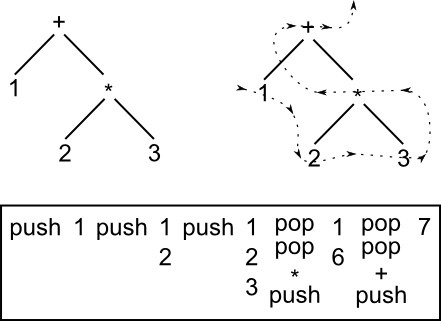
\includegraphics[width=.6\textwidth]{./img/arith.png}
    \caption{Árvore da expressão e operações resultantes na pilha.}
    \label{figure:example}
\end{figure}

O mesmo tipo de lógica foi implementado também para operadores booleanos e
permite a geração de código de forma mais simples, visto que já desenvolvemos
funções auxiliares para essas operações.

Apresentamos abaixo as operações principais da pilha aritmética. Todas as
outras operações da pilha se encontram no arquivo \verb!std.asm! no final do arquivo.


\begin{lstlisting}[frame=single,numbers=left,breaklines=true]
;--------------------------PUSH_ARITH------------------------------
PUSH_ARITH      JP /000
                MM TMP_1
                LD ARIT_PTR_STACK 
                +  TWO
                MM ARIT_PTR_STACK
                +  MOVE_CONST
                MM OP_PUSH_ARITH
                LD TMP_1
OP_PUSH_ARITH   JP /000 
                RS PUSH_ARITH 
;--------------------------POP_ARITH-------------------------------
POP_ARITH       JP /000 
                LD ARIT_PTR_STACK 
                -  TWO
                MM ARIT_PTR_STACK 
                +  TWO 
                +  LOAD_CONST 
                MM OP_POP_ARITH
OP_POP_ARITH    JP /000
                RS POP_ARITH 
;--------------------------SUM_ARITH-------------------------------
SUM_ARITH       JP /000 
                SC POP_ARITH
                MM TMP_2 
                SC POP_ARITH
                +  TMP_2 
                SC PUSH_ARITH
                RS SUM_ARITH 
;--------------------------MUL_ARITH-------------------------------
MUL_ARITH       JP /000 
                SC POP_ARITH
                MM TMP_2 
                SC POP_ARITH 
                *  TMP_2 
                SC PUSH_ARITH
                RS MUL_ARITH 
\end{lstlisting}


\section{Arrays e Structs}

Em \emph{CZAR} \textbf{não} existem \emph{Arrays} de tamanho dinâmico e sua criação está
limitada à declaração. Sendo assim, suas dimensões internas são conhecidas pelo
compilador a todo momento e seu cálculo de posição é facilitado e feito em
tempo de compilação. 

\begin{lstlisting}[frame=single,numbers=left,breaklines=true, language=C]
int i;

/* 
* Array int[4][3][2]: 
*
* [
*    [[0, 0], [0, 0], [0, 0]], 
*    [[0, 0], [0, 0], [0, 0]], 
*    [[0, 0], [0, 0], [0, 0]], 
*    [[0, 0], [0, 0], [0, 0]]
* ]
*
* Preenchendo com:
* ----------------
* decl int i;
* decl int j;
* decl int k;
* decl int l; 
* set i = 0;
* set j = 0;
* while (j < 4) {
*   set k = 0;
*   while (k < 3) {
*     set l = 0;
*     while (l < 2) {
*       set array_ex[j][k][l] = i;
*       set i = i + 1;
*       set l = l + 1;
*     }
*     set k = k + 1;
*   }
*   set j = j + 1;
* }
*
* Temos:
* ------
* [
*    [[0, 1], [2, 3], [4, 5]], 
*    [[6, 7], [8, 9], [10, 11]], 
*    [[12, 13], [14, 15], [16, 17]], 
*    [[18, 19], [20, 21], [22, 23]]
* ]
* ou:
* ---
* [
*   0, 1, 2, 3, 4, 5, 6, 7, 8, 9, 10,
*   10, 11, 12, 13, 14, 15, 16, 17, 18, 
*   19, 20, 21, 22, 23
* ]
*
*
*
*
*/
acc = acumulado[n_dimensoes - 1] = 1; // maybe long 1L 
for (i = n_dimensoes-2; i >= 0; i--) {
   acc = acumulado[i+1] = dimensoes[i+1] * acc;
}
/* 
   acumulado = [6, 2, 1];
*/
for (i = 0; i < n_dimensoes; i++) {
    acumulado[i] = acumulado[i] * size_cell; // celulas podem ter 
                                             // tamanho variavel
}
for (i = 0; i < n_dimensoes; i++) {
    fprints(str, " LV =%d ", acumulado[i]);
    cpy_to_lines_of_code(str);
    fprints(str, " * ARR_DIM_%d", acumulado[i]);
    cpy_to_lines_of_code(str);
    fprints(str, " +  ADDRS_ACCUMULATOR");
    cpy_to_lines_of_code(str);
    fprints(str, " MM ADDRS_ACCUMULATOR");
    cpy_to_lines_of_code(str);
}
\end{lstlisting}

O cálculo de \emph{structs} é resolvido em tempo de compilação. Uma vez que o
tamanho de cada parte da estrutura é conhecida em tempo de compilação, é
possível se fazer toda a aritmética de acesso via programação em \emph{C}. 

\begin{lstlisting}[frame=single,numbers=left,breaklines=true, language=C]
    int deslocamento_para_celula(struct_struct* vi_struct, int cell_to_access) {
        int sum_up_to_ptr = 0;
        for (i = 0; i < cell_to_access; i++) {
            sum_up_to_ptr += vi_struct->sizes[i];
        }
        return sum_up_to_ptr;
    }
\end{lstlisting}


\chapter{Exemplo de programa traduzido}
\label{chap:exemplo-programa}
	% !TEX encoding = UTF-8 Unicode

A fim de demonstrar tudo o que foi pensado como a maneira de traduzir os comandos de alto nível da nossa linguagem CZAR, nós traduzimos um programa simples de fatorial que permite visualizar e testar a nossa tradução.

Para isso, apresentamos o exemplo de programa escrito em três diferentes linguagens: (i) na nossa linguagem de alto nível CZAR; (ii) tradução para linguagem de máquina, utilizando as bibliotecas complementares \emph{std} e \emph{stdio}; (iii) tradução para linguagem de saída MVN.

\section{Exemplo de programa fatorial na linguagem de alto nível}
\label{sec:alto-nivel}

\lstinputlisting[frame=single,numbers=left,breaklines=true,morekeywords={main,const,int,char,string,void,return,for,struct,if,ref,float,else,and,or,not,true,false,%
    meth, decl, call, set}]{example_compiled/exemplo_fatorial.czar}

\section{Tradução do programa fatorial para linguagem de máquina}
\label{sec:traducao-asm}

\lstinputlisting[frame=single,numbers=left,breaklines=true,morekeywords={JP,JZ,JN,LV,LD,MM,SC,RS,HM,GD,PD,OS}]{example_compiled/exemplo_fatorial_gen.asm}

\section{Tradução do programa fatorial para linguagem de saída MVN}
\label{sec:traducao-mvn}

\lstinputlisting[frame=single,numbers=left,breaklines=true]{example_compiled/exemplo_fatorial_gen.mvn}


\postextual

\bibliography{bibliografia}

\end{document}
